\documentclass[10pt,twocolumn]{article}

\usepackage[utf8]{inputenc}
\usepackage[scaled]{helvet}
\renewcommand*\familydefault{\sfdefault}
\renewcommand{\familydefault}{\sfdefault}

\usepackage{amsfonts}	
\usepackage{graphicx}
\usepackage{url}
\usepackage{subfigure}
\usepackage{nopageno}
\usepackage{setspace}
\usepackage{bibspacing}
\usepackage[pdftex]{hyperref}
\usepackage{grffile}

\hyphenation{time-stamps}

\begin{document}
\sloppy

\title{
  On the Spectral Evolution of Large Networks \\ 
  PhD Thesis Proposal
}
\author {Jérôme Kunegis \\
  \small{Institute for Web Science and Technologies} \\
  \small{University of Koblenz-Landau} \\
  \texttt{kunegis@uni-koblenz.de}
}

\maketitle

\begin{abstract}
In my dissertation, I study the spectral evolution of large networks. My
main result is an interpretation of the spectrum and eigenvectors of
networks in terms of global and local effects. I argue and show that the
spectrum describes a network on the global level, whereas eigenvectors
describe a network at the local level.  I observe this behavior in over
one hundred network datasets from social networks, authorship networks,
feature networks, rating networks, link networks, folksonomies and other
types of networks.  
Based on the spectral evolution
model, I introduce two novel link prediction methods, one based on curve
fitting, and one on spectral extrapolation.  
As special cases I
present variants of all methods that apply to bipartite and signed
graphs.
\end{abstract}

\section{Introduction}
A certain number of machine learning and data mining problems
can be formulated as the analysis of large networks:  social networks,
hyperlink networks, citation graphs, rating graphs, trust networks,
communication networks, etc.  
In these settings, a prominent type of problem is given by link
prediction:  Learn where new edges will appear.  Link prediction can be
applied to recommender systems, to collaborative filtering methods, or
everytime edges or edge weights are to be predicted. 
Many different approaches have been proposed to the link prediction
problem. 

I study the link prediction problem taking an algebraic approach: Given a matrix
associated with a network, compute a matrix decomposition, giving
eigenvalues (the spectrum) and eigenvectors.  Common matrices are the
adjacency and Laplacian matrices; common decompositions are the
eigenvalue and singular value decompositions.
Studying a large collection of network datasets I made the following
observations: 
\begin{itemize}
  \item Over time, the eigenvalues increase, while the
    eigenvectors stay approximately constant.
  \item The eigenvector components follow certain distributions
    (e.g. lognormal), and do not change significantly with time. 
\end{itemize}

These observations lead to two novel link prediction algorithms, one
based on curve fitting and one based on extrapolation.  I show that both
algorithms are competitive in many settings. 

The methods I present are very general and also apply to networks with
special structure and additional features.  In bipartite networks, I
use the biadjacency matrix instead of the adjacency matrix, leading
to odd pseudokernels.  In signed graphs, I use the signed
Laplacian matrix, giving signed spectral link prediction.  As a 
benefit, the signed Laplacian can be used for signed clustering. 

\section{Datasets}
During my research I have collected network
datasets~\cite{kunegis:network-survey}.  These datasets 
are either unipartite (such as social networks) or bipartite (such as
rating networks).  Some networks have edge weights, e.g. ratings or
trust/distrust links, in which case the link prediction problem also
consists of predicting the weight of edges.  Edge weights admit negative
values in some datasets. 
The networks include social networks, citation
graphs, hyperlink graphs, trust networks, rating graphs (i.e. user-item
graphs), communication graphs and others.  
Many of these graphs are used
in previous literature in various machine learning and data mining
subfields.  
Edges in some datasets additionally have timestamps. 
Figure~\ref{fig:sizes} gives an overview of the networks by
their size. 

\begin{figure}
  \centering
  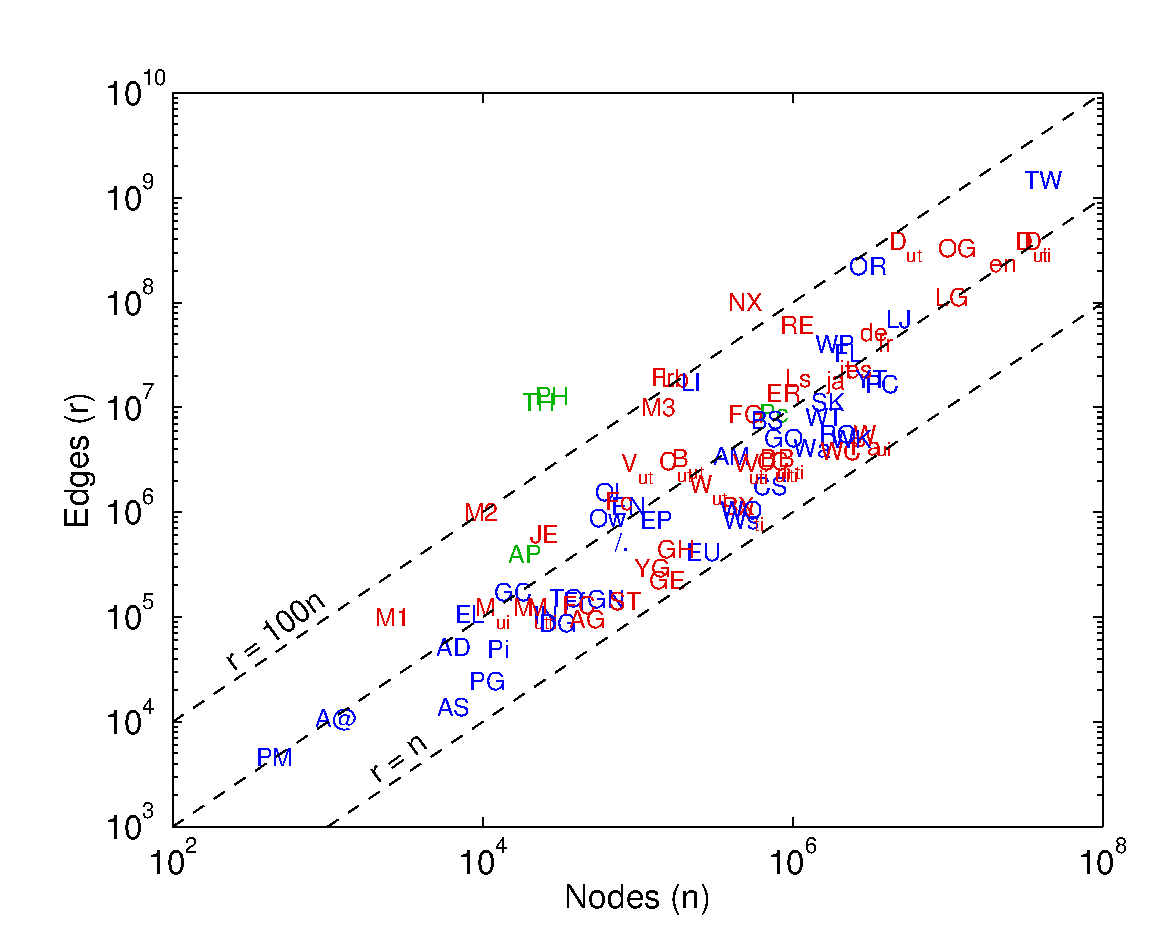
\includegraphics[width=.48\textwidth]{scatter.network-survey-relationships.a}
  \caption{
    Datasets from my dissertation arranged by total number of nodes and edges. 
    Unipartite networks are shown in red and bipartite networks in
    blue. 
  }
  \label{fig:sizes}
\end{figure}
I extracted one dataset myself, and studied it
separately:  the Slashdot Zoo~\cite{kunegis:slashdot-zoo}. 
This dataset has the distinction of
containing negative edge weights in a social network. 

The following is a sample of datasets used.  A longer list is given
in~\cite{kunegis:network-survey}. 
\begin{itemize}
  \item Unipartite unweighted datasets:  hep-th citations~\cite{b352},
    the WWW link graph~\cite{b396},
    the Advogato trust network~\cite{b334}, Patentcite
    citations~\cite{b376}, DBLP citations~\cite{b525}, TREC WT10G 
    hyperlinks~\cite{b397}, Citeseer citations~\cite{b524}, Twitter
    followers~\cite{b545}, English Wikipedia hyperlinks~\cite{download.wikimedia.org}, Facebook 
    friends and wall posts~\cite{b421}.
  \item Unipartite weighted datasets:  the Slashdot Zoo~\cite{kunegis:slashdot-zoo},
    LíbímSeTi dating site ratings~\cite{b311}, Epinions~\cite{b325}, Enron e-mails~\cite{b431}.
  \item Bipartite unweighted networks: DBLP authorship~\cite{b525}, CiteUlike tags~\cite{b349},
    English Wikipedia categories~\cite{download.wikimedia.org}, the edit
    networks of several language
    Wikipedias~\cite{download.wikimedia.org}, BibSonomy user/item/tag
    networks~\cite{b346}, Delicious user/item/tag 
    networks~\cite{wetzker2008a}. 
  \item Bipartite weighted networks:  Reuters~\cite{b553}, MovieLens
    (several sizes)~\cite{www.grouplens.org/node/73}, 
    Netflix~\cite{b520}, Book Crossing (BX)~\cite{b523}, Jester~\cite{b7}. 
\end{itemize}

\section{Algebraic Graph Theory}
My analysis of networks is based on algebraic graph theory~\cite{b285}.
I study the decomposition of certain matrices associated with graphs.
The (weighted) edge set of a graph can be represented by a matrix whose
characteristics follow those of the graph.  Unweighted graphs lead to a
0/1 matrix, undirected graphs to a symmetric matrix, bipartite graphs to
a rectangular matrix, and so on.  This matrix is called the adjacency
matrix and is denoted $A$.  The following decompositions can be
computed:
\begin{itemize}
  \item Singular value decomposition:  $A = U\Sigma V^T$
  \item Eigenvalue decomposition:  $A+A^T = U\Lambda U^T$
  \item Eigenvalue decomposition of the Laplacian matrix:  $L =
    U\Lambda U^T$
\end{itemize}
The columns $U$ and $V$ are the (Laplacian) eigenvectors of the
network.  $\Sigma$  and $\Lambda$ are the spectra of the network,
containing the singular values and eigenvalues.  

My thesis consists of studying the behavior of $U$, $V$, $\Sigma$ and
$\Lambda$ of networks as these grow. 
While studying the Laplacian matrix of weighted networks, I found a way
of defining it for networks with negative edge
weights~\cite{kunegis:negative-resistance,kunegis:netflix-srd,kunegis:signed-kernels}. 

\section{Link Prediction}
Many machine learning problems applying to networks can be understood as
\emph{link prediction}.  The two main problems are: predicting where
links will appear~\cite{b256} and predicting the weight of new edges, if
edges are weighted (e.g. collaborative filtering~\cite{b25}, predicting
trust~\cite{b325}, friendship/enmity prediction~\cite{kunegis:slashdot-zoo}).
By studying the evolution of networks over time I made the following
observations:
\begin{itemize}
\item Eigenvectors remain largely constant over time
\item Spectra evolve over time
\end{itemize}
These lead to link prediction algorithms that compute a new spectrum and
multiply it with the known eigenvectors to predict links.  It turns out
that several common link prediction methods are of this form, using
various ways of transforming the spectrum~\cite{b191,b137,b156,b155}.
To learn a good spectral transformation, two methods can be used:
\begin{itemize}
  \item Extrapolate the growth of the eigenvalues over
    time~\cite{kunegis:spectral-network-evolution}, see 
    Figures~\ref{subfig:time_spectrum} and~\ref{subfig:evol_permutation_map}. 
  \item Reduce the problem to a one-dimensional curve fitting
    problem~\cite{kunegis:spectral-transformation}, see
    Figure~\ref{subfig:curve}.  
\end{itemize}

\begin{figure}[h!]
  \centering
    \subfigure[Spectral growth]{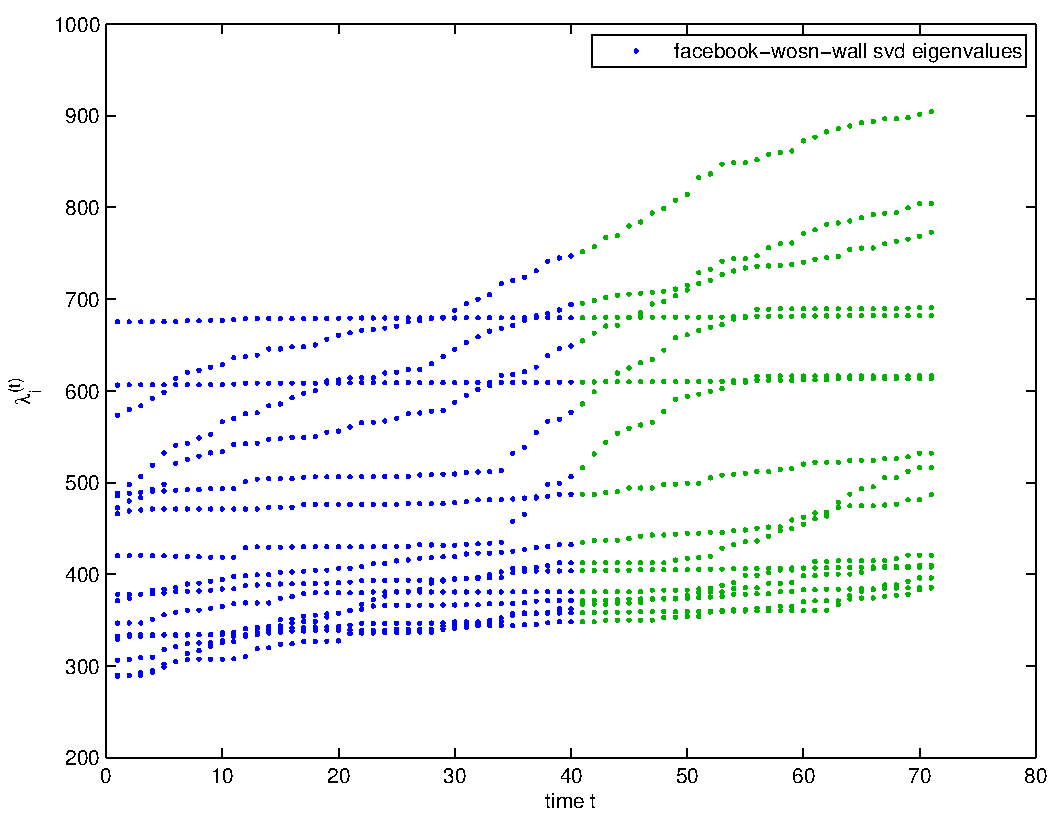
\includegraphics[width=.26\textwidth]
      {time_spectrum} \label{subfig:time_spectrum}}
    \subfigure[Eigenvector
      similarity]{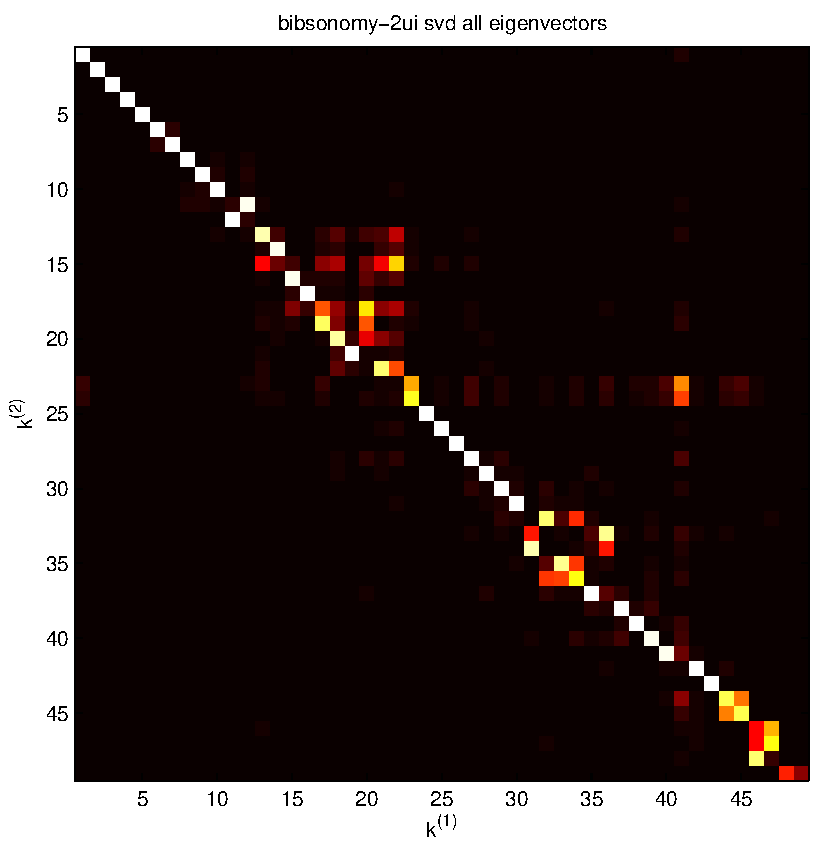
\includegraphics[width=.25\textwidth]
      {evol_permutation_map:svd:bibsonomy-2ui:uv} \label{subfig:evol_permutation_map}}
    \subfigure[Learning a spectral transformation]
              {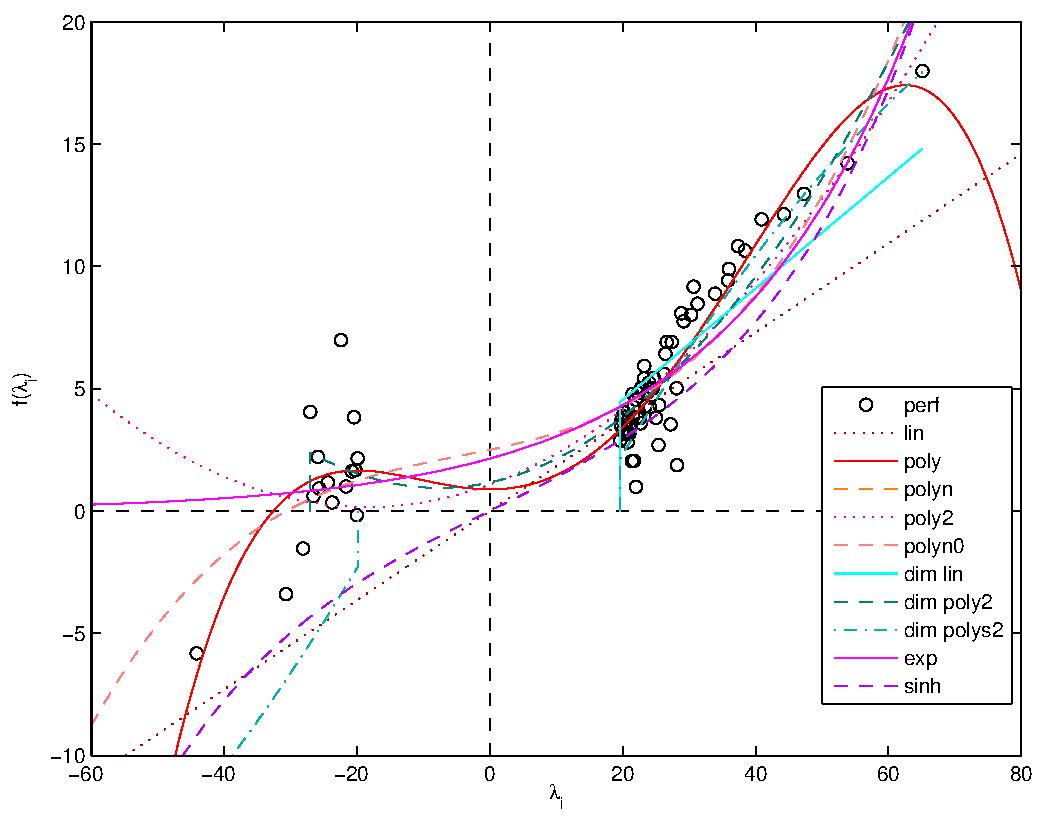
\includegraphics[width=.26\textwidth]{curve} \label{subfig:curve}} 
  \caption{
    Link prediction methods:  
    (a) Evolution of the singular values in the Facebook wall post
    network.  The evolution of the spectrum on the right part (in
    green) can be extrapolated from the known spectral evolution on the
    left (in blue).
    (b) Cosine distance between current and expected eigenvectors in the
    BibSonomy user-item graph.  (white = 1, black = 0)  This shows that
    indeed most eigenvectors remain the same, although a few do not.
    This plot also shows that some eigenvalue \emph{pass} others.
    (c) Curve fitting current and expected spectrum in the hep-th
    citation network, using the method described in~\cite{kunegis:spectral-transformation}. 
    }
\end{figure}
I evaluated these two methods on the collection of large network
datasets, and found they are both competive in all kinds of link
prediction tasks, over all types of network types. 

\section{Current State}
Preliminary results of my work were published as conference papers.

I began my research by studying the collaborative filtering problem.  In
particular, I applied the Laplacian matrix to networks with
negative edge
weights~\cite{kunegis:negative-resistance,kunegis:netflix-srd,kunegis:signed-kernels}.   
That last and most complete analysis was presented at SIAM SDM 2010. 

An analysis of the self-acquired Slashdot Zoo dataset containing
positive and negative edges between users (``friends'' and ``foes'') was
presented separately at WWW 2009~\cite{kunegis:slashdot-zoo}. 

My work on graph kernels started by studying their scalability and their
application as similarity
functions~\cite{kunegis:alternative-similarity,kunegis:kernel-scalability}.
In a later paper I introduced a method for learning spectral
transformations~\cite{kunegis:spectral-transformation} (presented at
ICML 2009).  
An empirical verification of the spectral evolution model, along with
the spectral extrapolation algorithm will be presented at CIKM
2010~\cite{kunegis:spectral-network-evolution}. 

A survey of the network datasets I collected was written and submitted
to ICDM 2010~\cite{kunegis:network-survey}. 

\section{Future Work}
While these tasks are not part of my dissertation, they follow directly
from it.
\begin{itemize}
\item Application of spectral learning to other, more complex matrix
  decompositions:  nonnegative matrix factorization, approximations with
  missing data (e.g.~\cite{b178}), probabilistic latent semantic
  analysis, maximum margin matrix factorization.
\item Studying link prediction in networks with multiple vertex and node
  types, leading to new machine learning problems, such as learning
  relative weights of different edge types. 
\item Characterizing graphs based on the spectrum and a probability
  distribution for eigenvectors. 
\end{itemize}

\bibliographystyle{acm}
\bibliography{kunegis}

\end{document}
